\chapter{Conceptual Framework}
\label{sec:conceptual-framework}

\begin{figure}[htbp]
    \centering
    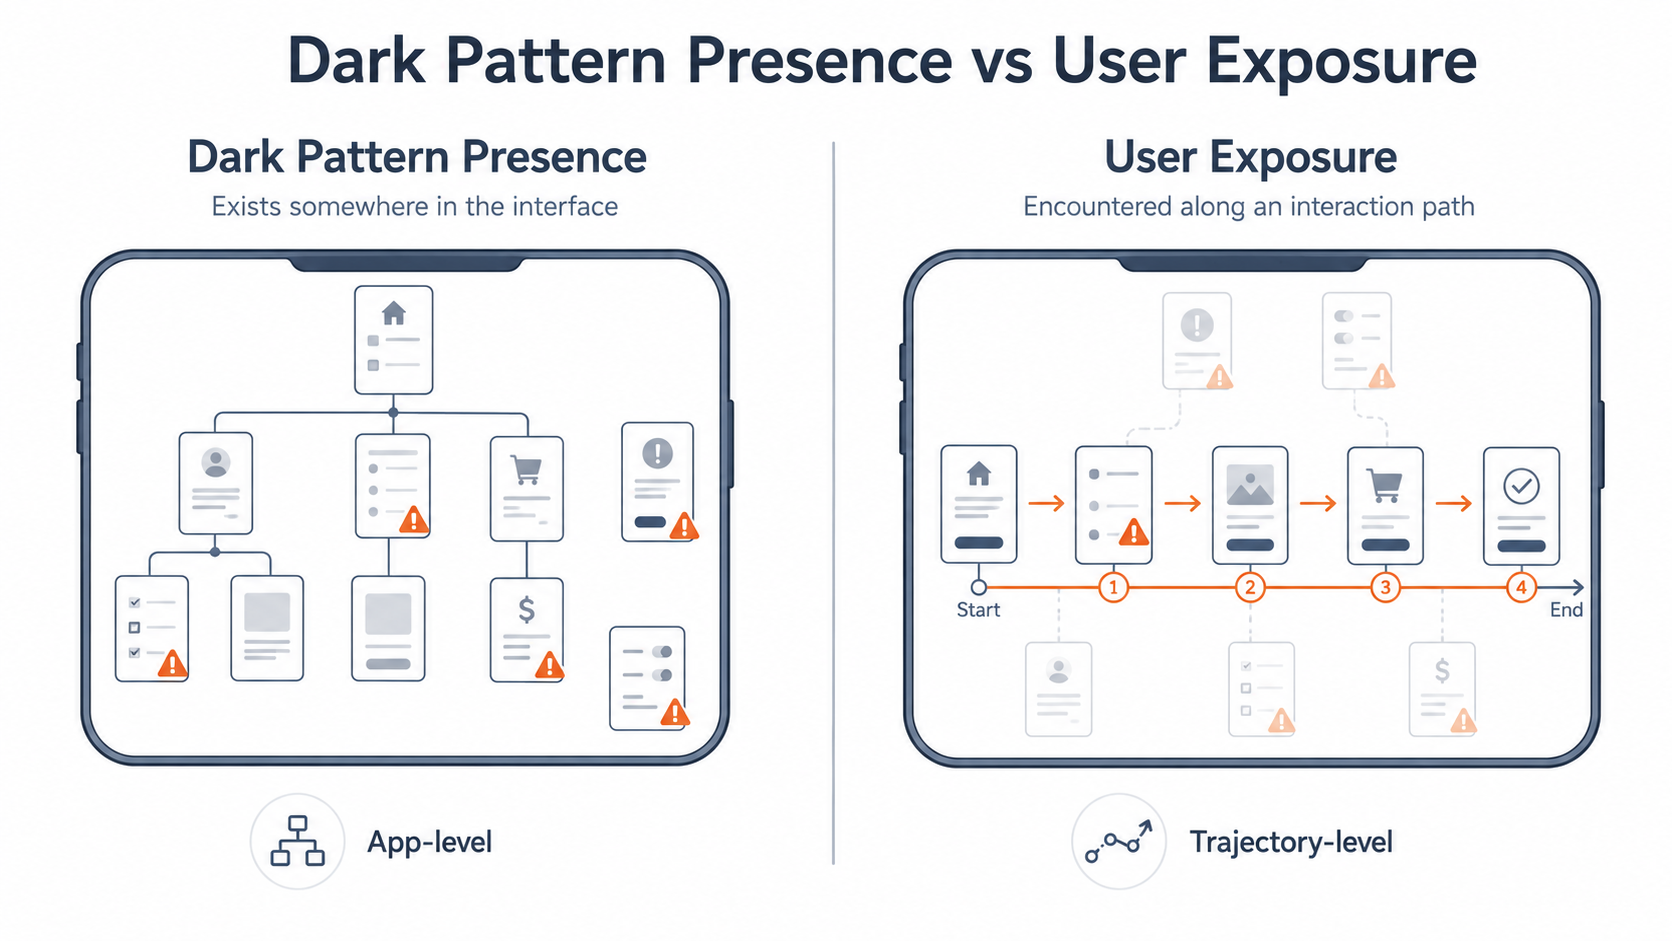
\includegraphics[width=0.95\linewidth]{figures/pictures/presence_vs_exposure.png}
    \caption{Presence vs. Exposure}
    \label{fig:presence_vs_exposure}
\end{figure}


\section{Interface Presence vs. User Exposure}
\label{subsec:presence-exposure}

A central conceptual distinction in this project is the difference between the \emph{presence} of a dark pattern and a user's \emph{exposure} to that dark pattern. Existing studies on deceptive user interfaces have made substantial progress in identifying, categorizing, and measuring dark patterns in websites, mobile applications, and consent interfaces \cite{gray2018darkpatterns,mathur2019darkpatterns,mathur2021whatmakesdark}. In these studies, a dark pattern is often treated as an interface element, design strategy, or choice architecture mechanism that exists somewhere in a digital system. Under this view, a dark pattern is considered present if an application contains, for example, a misleading button, a difficult cancellation path, a countdown timer, a hidden charge, a nagging pop-up, or a forced registration requirement.

However, interface presence alone does not fully describe what users actually experience. A dark pattern may exist in an application but may not be encountered by every user. Some deceptive interface mechanisms appear only after a user searches for a certain keyword, opens a recommended item, enters a payment page, clicks a promotion, or attempts to reject an offer. Others may appear only in specific task flows, such as membership subscription, coupon redemption, food ordering, or checkout confirmation. Therefore, an application-level statement such as ``this app contains a dark pattern'' is informative but incomplete. It indicates that a problematic interface mechanism exists, but it does not indicate whether a particular user profile is likely to encounter it during interaction.

This report therefore shifts the unit of analysis from \emph{dark pattern presence} to \emph{dark pattern exposure}. Exposure refers to the event in which a user actually reaches and observes a dark pattern during an interaction process. In this sense, exposure is conditional on user behavior, search keywords, interface transitions, and the application's response to those actions. This distinction is especially important in mobile applications, where interfaces are dynamic, task-oriented, and often influenced by recommendation or personalization mechanisms. The same application may expose different users to different screens, not necessarily because of explicit demographic targeting, but because different interests and behaviors guide users into different regions of the interface space.

The concept of \emph{differential exposure} further extends this distinction. Differential exposure occurs when different controlled user profiles encounter different types or levels of dark pattern exposure under comparable experimental conditions. For example, a high-payment shopping profile may more frequently reach checkout pages, membership prompts, and urgency-based promotions, while a low-payment browsing profile may remain closer to feeds, homepage browsing, and general content exploration. If their observed DPS annotations differ systematically, the result suggests that dark pattern exposure is associated with profile-conditioned interaction behavior. Importantly, this does not by itself prove intentional targeting by the platform. Rather, it provides empirical evidence that different profiles may experience different observable exposure patterns.

\section{Interaction Trajectories}
\label{subsec:interaction-trajectories}

To analyze exposure rather than mere presence, this project models mobile app usage as an interaction trajectory. A trajectory records the sequence of actions performed by a controlled profile, the interface states reached after those actions, and the dark pattern annotations assigned to the corresponding screenshots. Before defining the trajectory, we first define a simplified action space:

\begin{equation}
\mathcal{A}
=
\{\mathrm{home}, \mathrm{search}, \mathrm{browse}, \mathrm{decision}\}.
\label{eq:action-space}
\end{equation}

Here, $\mathcal{A}$ denotes the set of possible interaction actions used in the conceptual framework. The action $\mathrm{home}$ represents homepage visits or returning to the main interface, $\mathrm{search}$ represents keyword-based search, $\mathrm{browse}$ represents scrolling or opening ordinary content, and $\mathrm{decision}$ represents entering decision-related interfaces such as checkout, subscription, ordering, or confirmation pages. This four-category abstraction is the conceptual action space used throughout the analysis.

The implementation layer may instantiate these categories with a finer-grained action set, such as:

\begin{itemize}
    \item \texttt{visit\_homepage}
    \item \texttt{search\_keyword}
    \item \texttt{browse\_or\_scroll\_page}
    \item \texttt{click\_recommended\_item}
    \item \texttt{like\_or\_favorite}
    \item \texttt{follow\_account}
    \item \texttt{stay\_on\_content}
    \item \texttt{decision\_interface\_visit}
    \item \texttt{close\_popup}
    \item \texttt{back}
\end{itemize}

These implementation-level actions are mapped back to the four conceptual categories before exposure analysis, so the mathematical definitions below remain unchanged while the operational traces can stay more detailed.

Each controlled user profile is represented by two components:

\begin{equation}
A_i = (C_i, B_i),
\label{eq:profile-definition}
\end{equation}

where $A_i$ denotes the $i$-th user profile, $C_i$ denotes the keyword preference distribution of that profile, and $B_i$ denotes its behavior or action distribution. In other words,

\begin{equation}
C_i : \text{keyword preference distribution},
\label{eq:keyword-distribution-text}
\end{equation}

\begin{equation}
B_i : \text{behavior/action distribution}.
\label{eq:behavior-distribution-text}
\end{equation}

The keyword distribution describes what the profile tends to search for, while the behavior distribution describes how the profile tends to interact with the application. For example, a bargain-hunter profile may assign higher probability to keywords such as discounts, coupons, flash sales, or group-buying, while a high-payment shopping profile may assign higher probability to high-value product keywords. Similarly, the high-payment profile may be more likely to enter decision-related interfaces, whereas the low-payment browsing profile may be more likely to browse or scroll.

The behavior distribution of profile $A_i$ is defined as

\begin{equation}
\pi_{A_i}(a)
=
P(a_t = a \mid A_i),
\qquad a \in \mathcal{A}.
\label{eq:behavior-probability}
\end{equation}

This equation means that $\pi_{A_i}(a)$ is the probability that profile $A_i$ performs action $a$ at interaction step $t$. Since $\pi_{A_i}$ is a probability distribution over the action space, it must satisfy

\begin{equation}
\sum_{a \in \mathcal{A}} \pi_{A_i}(a) = 1.
\label{eq:behavior-normalization}
\end{equation}

Similarly, the keyword preference distribution of profile $A_i$ is defined as

\begin{equation}
\rho_{A_i}(w)
=
P(k_t = w \mid A_i, a_t = \mathrm{search}),
\qquad w \in \mathcal{K}_{A_i}.
\label{eq:keyword-probability}
\end{equation}

Here, $k_t$ denotes the keyword selected at step $t$, $w$ denotes a candidate keyword, and $\mathcal{K}_{A_i}$ denotes the keyword set associated with profile $A_i$. This equation means that when profile $A_i$ performs a search action, the keyword is sampled from its profile-specific keyword distribution. The keyword distribution also satisfies a normalization condition:

\begin{equation}
\sum_{w \in \mathcal{K}_{A_i}} \rho_{A_i}(w) = 1.
\label{eq:keyword-normalization}
\end{equation}

At each interaction step, the action is sampled from the profile-conditioned behavior distribution:

\begin{equation}
a_t \sim \operatorname{Categorical}(\pi_{A_i}).
\label{eq:action-sampling}
\end{equation}

This means that the next action is not chosen arbitrarily, but is generated according to the behavioral tendency of the corresponding profile. If the sampled action is search, then the keyword is sampled from the profile-conditioned keyword distribution:

\begin{equation}
k_t \sim \operatorname{Categorical}(\rho_{A_i})
\qquad
\text{if } a_t = \mathrm{search}.
\label{eq:keyword-sampling}
\end{equation}

These equations provide a simple probabilistic model of profile-conditioned interaction. They do not attempt to learn the full behavior of real users. Instead, they define controlled and reproducible profile behaviors for audit experiments. This is suitable for the purpose of the project because the objective is not to infer real user identities or demographic attributes, but to examine whether different controlled behavioral profiles are associated with different dark pattern exposure.

Based on this action generation process, the interaction trajectory of profile $A_i$ is defined as

\begin{equation}
\tau_{A_i}
=
\big(
(a_1, s_1, d_1),
(a_2, s_2, d_2),
\ldots,
(a_T, s_T, d_T)
\big),
\label{eq:trajectory}
\end{equation}

where $a_t$ is the action performed at step $t$, $s_t$ is the resulting interface state or screenshot, $d_t$ is the DPS annotation assigned to that state, and $T$ is the interaction budget. In this project, $T$ is fixed at 30 steps for each app-profile pair. The trajectory therefore connects three components: the action generated by the profile, the interface state returned by the application, and the dark pattern exposure observed in that state.

The annotation $d_t$ is represented as a seven-dimensional DPS vector:

\begin{equation}
d_t
=
[I_t, F_t, P_t, C_t, S_t, N_t, FA_t],
\label{eq:dps-vector-step}
\end{equation}

where $I_t$ denotes Interface Interference, $F_t$ denotes Friction, $P_t$ denotes Pressure, $C_t$ denotes Contextual Deception, $S_t$ denotes Sneaking, $N_t$ denotes Nagging, and $FA_t$ denotes Forced Action at step $t$. This trajectory-based view is important because dark pattern exposure is often sequential. Friction may appear only when the user attempts to reject or cancel an option. Pressure may appear after the user enters a shopping or payment context. Forced action may appear when the user cannot proceed without logging in, granting permission, or accepting a membership prompt. A single static screenshot may miss these mechanisms, while an interaction trajectory can capture how exposure accumulates across repeated app usage.

\begin{figure}[htbp]
    \centering
    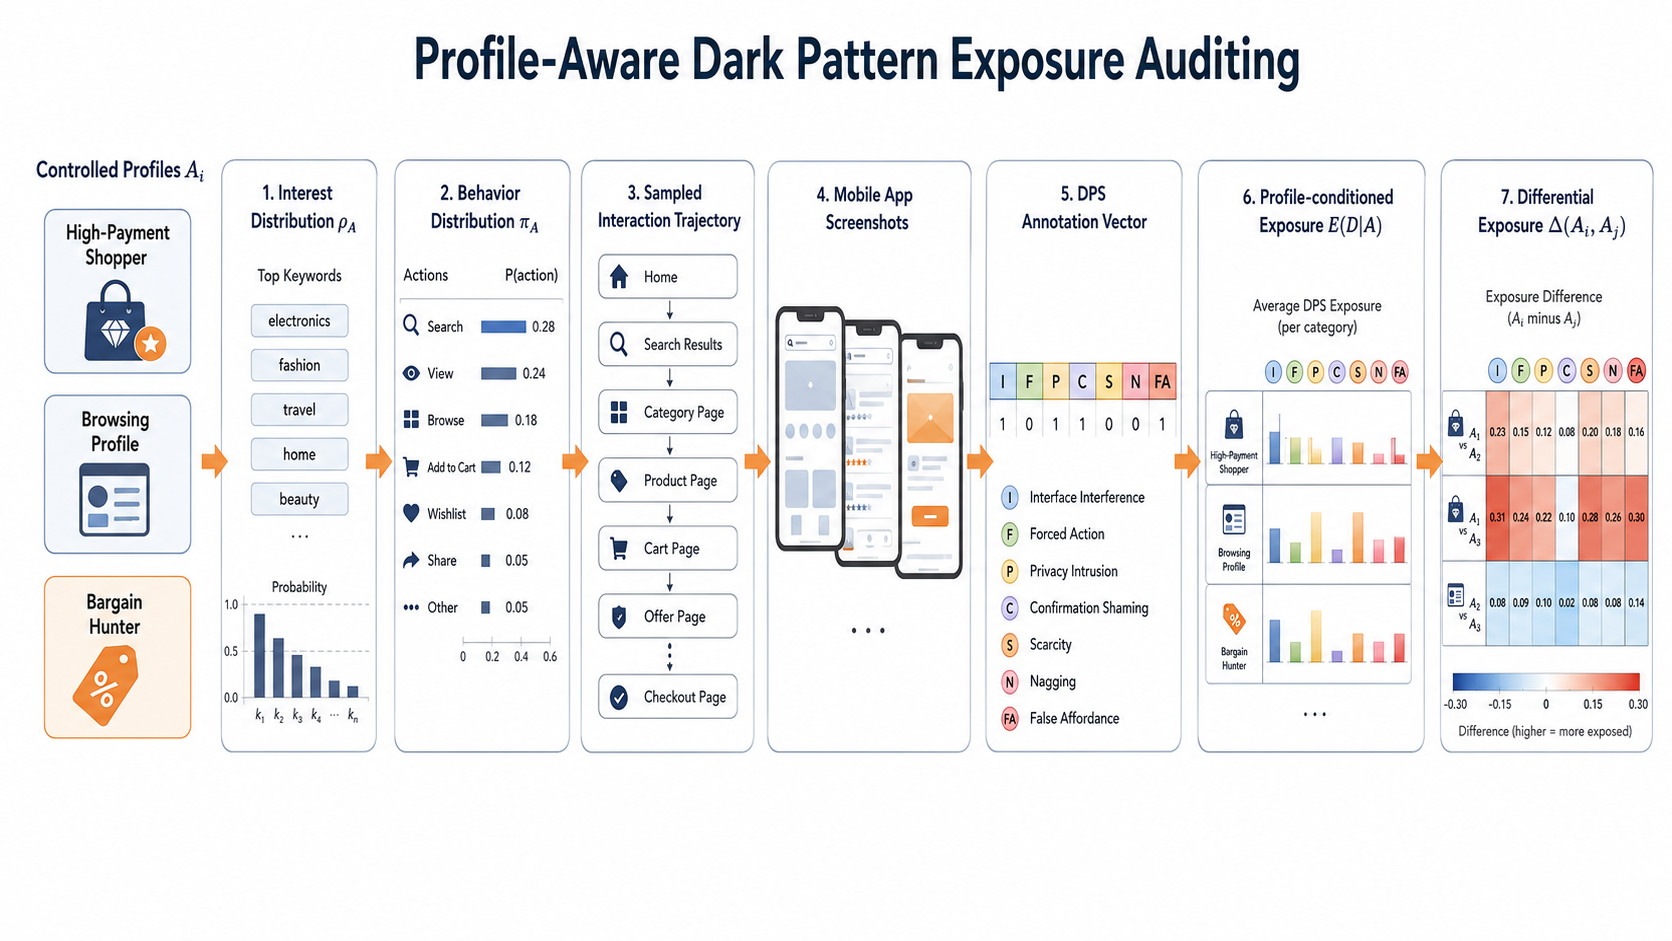
\includegraphics[width=0.95\linewidth]{figures/pictures/core_conceptual_framework.png}
    \caption{Core Conceptual Framework}
    \label{fig:core_conceptual_framework}
\end{figure}

\section{Profile-conditioned Exposure}
\label{subsec:profile-conditioned-exposure}

Based on the trajectory representation, this project defines profile-conditioned dark pattern exposure as

\begin{equation}
E(D \mid A_i),
\label{eq:conditional-exposure}
\end{equation}

where $D$ denotes dark pattern exposure and $A_i$ denotes a controlled user profile. This expression represents the expected or average dark pattern exposure observed under profile $A_i$. Since exposure is annotated using the seven-dimensional DPS vector, the profile-conditioned exposure is also represented as a seven-dimensional vector:

\begin{equation}
E(D \mid A_i)
=
\big[
E(I \mid A_i),
E(F \mid A_i),
E(P \mid A_i),
E(C \mid A_i),
E(S \mid A_i),
E(N \mid A_i),
E(FA \mid A_i)
\big].
\label{eq:conditional-exposure-vector}
\end{equation}

This equation means that the exposure of a profile is not reduced to a single undifferentiated number. Instead, it preserves the type of exposure. Two profiles may have similar overall exposure levels but may encounter different dark pattern mechanisms. For example, one profile may experience more Interface Interference and Pressure, while another may experience more Friction or Forced Action. The vector form makes it possible to compare exposure at the level of individual mechanisms rather than only through total counts.

Empirically, $E(D \mid A_i)$ is estimated by averaging the DPS annotations collected along the interaction trajectories of profile $A_i$. If the profile is tested across multiple applications and multiple steps, the empirical estimate can be written as

\begin{equation}
\widehat{E}(D \mid A_i)
=
\frac{1}{|\mathcal{R}_i|}
\sum_{r \in \mathcal{R}_i} d_r,
\label{eq:empirical-conditional-exposure}
\end{equation}

where $\mathcal{R}_i$ denotes the set of interaction records collected under profile $A_i$, and $d_r$ denotes the DPS vector of record $r$. The hat symbol in $\widehat{E}$ indicates that this is an empirical estimate based on observed data rather than a theoretical expectation known in advance.

This interpretation is important for avoiding causal overclaiming. A higher value of $\widehat{E}(P \mid A_i)$ indicates that profile $A_i$ encountered more pressure-related interface states in the collected audit records. It does not necessarily prove that the application intentionally targeted that profile with pressure mechanisms. The observed pattern may result from recommendation logic, search results, commercial interface design, task flow structure, or the fact that certain profiles enter more decision-sensitive contexts. Therefore, profile-conditioned exposure should be understood as an empirical measure of observed exposure under controlled audit conditions, not as direct evidence of platform intent.

\section{Differential Exposure}
\label{subsec:differential-exposure}

After estimating exposure for each profile, the next step is to compare profiles. Differential exposure between two profiles $A_i$ and $A_j$ is defined as

\begin{equation}
\Delta(A_i, A_j)
=
E(D \mid A_i) - E(D \mid A_j).
\label{eq:differential-exposure}
\end{equation}

This equation defines differential exposure as the difference between two profile-conditioned exposure vectors. Since both $E(D \mid A_i)$ and $E(D \mid A_j)$ are seven-dimensional vectors, $\Delta(A_i, A_j)$ is also a seven-dimensional vector:

\begin{equation}
\Delta(A_i, A_j)
=
[
\Delta I,
\Delta F,
\Delta P,
\Delta C,
\Delta S,
\Delta N,
\Delta FA
].
\label{eq:differential-exposure-vector}
\end{equation}

Each component of this vector corresponds to one DPS dimension. A positive value in $\Delta I$ means that profile $A_i$ encountered more Interface Interference than profile $A_j$ on average. A negative value in $\Delta FA$ means that profile $A_i$ encountered less Forced Action than profile $A_j$ on average. In this way, the difference vector reveals not only whether two profiles differ, but also which dark pattern mechanisms account for the difference.

For example, comparing the high-payment shopping profile with the low-payment browsing profile may indicate whether stronger purchase-oriented behavior is associated with greater exposure to promotional pressure, interface interference, or payment-related forced action. Comparing the bargain-hunter profile with the high-payment shopping profile may show whether discount-oriented behavior is associated with urgency messages, coupon prompts, or membership restrictions. These comparisons move beyond the question of whether an application contains dark patterns and instead ask which profile encounters which mechanisms during interaction.

In addition to the signed difference vector, the overall distance between two exposure vectors can be measured using the $L_1$ distance:

\begin{equation}
L_1(A_i, A_j)
=
\sum_{m=1}^{7}
\left|
E(D_m \mid A_i) - E(D_m \mid A_j)
\right|,
\label{eq:l1-distance}
\end{equation}

where $D_m$ denotes the $m$-th dimension of the DPS vector. This equation sums the absolute differences across all seven DPS dimensions. A larger $L_1$ distance indicates a larger overall separation between the exposure patterns of two profiles, while a smaller value indicates more similar exposure patterns. Unlike the signed vector $\Delta(A_i, A_j)$, the $L_1$ distance does not indicate which profile has more exposure in a particular dimension. Instead, it provides a compact measure of the magnitude of the overall difference.

Together, $\Delta(A_i, A_j)$ and $L_1(A_i, A_j)$ provide complementary views of differential exposure. The difference vector is useful for interpretation because it identifies which dark pattern mechanisms vary across profiles. The $L_1$ distance is useful for summarizing the overall strength of the difference. In the later analysis, these measures can be combined with heatmaps, running mean convergence curves, permutation tests, q-values, and association measures such as Cramér's V to evaluate whether observed profile differences are stable and statistically meaningful.

This conceptual framework establishes the analytical bridge between controlled profile behavior and measurable dark pattern exposure. Rather than treating dark patterns only as static interface artifacts, it treats exposure as a trajectory-based, profile-conditioned, and empirically estimable outcome. The next section builds on this framework by explaining how the controlled profiles are constructed through interests and behaviors while excluding demographic attributes.
